\section{Computational Experiment}

%TODO: The main section of the report. Describe and motivate the choice of tools and the distributed system that you designed. Describe how you have designed your scalability experiments,and present the results.

This section provides the motivation for our choice of tools and briefly describes the distributed system that we designed. 

\subsection{Why Spark}
Spark provides a new model of computation that allows to perform multiple parallel operations on a specific set of data. In our project we apply multiple functions repeatedly to the same data set to extract various statistical information, hence Spark offers the possibility to improve significantly our performances without reloading each time the data form disk\cite{Sparkzaharia}.

Our dataset is spread among a read-only collection of objects called RDD, those objects allow parallel operations with the option of caching an RDD in memory so it can be reused for other MapReduce operations. An RDD does not exist in physical storage but it is computed from data in the reliable storage. 
RDDs can be constructed in four ways, we choose to construct it from a \textit{.csv} file in a shared file system. The System we have is fault tolerant, in fact if a partition of an RDD is lost it is possible to rebuild just that partition given the information on how it was derived from other RDDs. This is called \textit{lineage}\cite{Sparkzaharia}.

The system in use overcomes the inefficiency of other frameworks for accessing a cluster's computational resources, that is, it makes it possible to reuse intermediate results across multiple computations\cite{RDD}. \\
In our system a \textit{driver program} connects to a cluster of \textit{workers}, these are processes that can store RDD partitions in RAM across operations\cite{RDD}. 

\subsection{Results}
For this project, we are using Crimes dataset\cite{cityOfChicago} from city of chicago portal and it contains many relevant information associated with each of the crime that has occurred in Chicago from year 2001 until now. We are plotting 4 different graphs associated with 4 different columns. A program in pyspark was created to plot these graph. You can look at the code \href{https://github.com/ankurshukla03/ldsaproject/blob/edit_report/code/Crimes.ipynb}{here.} \\
Below is 4 different plots presenting the results :\\

\mfigure{crime_type}{Plot representing the number of times a particular crime type has occured in Chicago from year 2001 until now.}

\mfigure{month}{Plot representing the frequency of crime across the months.}

\mfigure{year}{Plot representing the frequency of crime per year.}

\mfigure{location}{Plot repersenting the frequency of crime with location description.}

\subsection{Scalability experiment}
In order to test and confirm the scalability of the system, scalability studies were conducted. Since the original dataset was only 1,45 GB, it was scaled up by replicating it in order to get larger datasets. Four different sizes of the dataset were produced including the original one. These were 1.45 Gb, 11.2 Gb, 23.2 Gb and 35 Gb and you can see the time taken with different number of nodes on these data size in Table \ref{table_time}.

To measure the horizontal scalability, the run time for a specific job on the dataset were recorded for 1 to 3 nodes in the cluster. As seen in  \ref{fig:scalabilityGraph} below we can observe that
the run time increased linearly with data size for the different cluster configurations and the run time was reduced equally for increasing number of nodes. Furthermore, the slopes for the linear fits of the data points are shown. The slope for one node is 41.241 s/GB and for four nodes it is 13.114 s/GB. This means that the second configuration is 3,15 times faster.\\

\begin{table}[]
    \centering
    \begin{tabular}{|c|c|c|}
\hline
Number of Nodes  & Time Taken & Data Size \\ \hline
        1 & 1.1 min & 1.45 Gb \\ \hline
        3 & 32 seconds & 1.45 Gb \\
\hline
\end{tabular}
\quad
\begin{tabular}{|c|c|c|}
\hline
Number of Nodes  & Time Taken & Data Size \\ \hline
        1 & 4.1 min & 5.8 Gb \\ \hline
        3 & 1.4 min & 5.8 Gb \\
\hline
\end{tabular}
\begin{tabular}{|c|c|c|}
\hline
Number of Nodes  & Time Taken & Data Size \\ \hline
        1 & 16 min & 23.2 Gb \\ \hline
        3 & 5.1 min & 23.2 Gb \\
\hline
\end{tabular}
\quad
\begin{tabular}{|c|c|c|}
\hline
Number of Nodes  & Time Taken & Data Size \\ \hline
        1 & 24 min & 35 Gb \\ \hline
        3 & 7.6 min & 35 Gb \\
\hline
\end{tabular}
    \caption{Time taken by different number of nodes on different data size. We are writing here only the time taken by reduce functionality as it is so large compare to other functions that it has a significant role while computing time taken by our code as you can see in figure \ref{fig:stages_one_fourth}.}
    \label{table_time}
\end{table}


\mfigure{stages_one_fourth}{Screenshot of our Spark UI stages tab when ran with 1 node on 35 Gb data size.}

\mfigure{stages_three_second}{Screenshot of our Spark UI stages tab when ran with 3 node on 5.8 Gb data size.}

\mfigure{stages_three_fourth}{Screenshot of our Spark UI stages tab when ran with 3 worker node on 35 Gb data size.}

\begin{figure}[H]
    \centering
    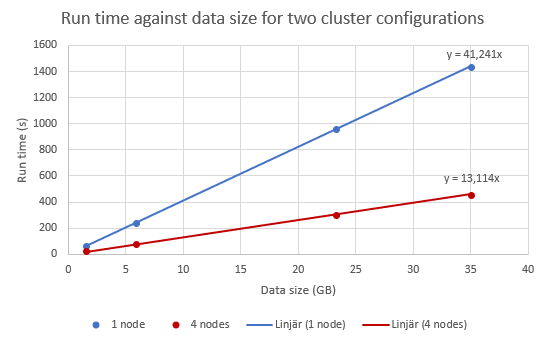
\includegraphics[width=.75\linewidth]{figures/runTime.PNG}
    \caption{Run time for different data sizes plotted for two cluster configurations. Blue line is the cluster with one node and the red line is with three nodes.}
    \label{fig:scalabilityGraph}
\end{figure}


\subsection{System Design}





